\documentclass[a4paper]{article}
\title{MAT257---Analysis 2}
\author{Jonah Chen}

\usepackage[utf8]{inputenc}
\usepackage[margin=0.5in]{geometry}

\usepackage{braket}
\usepackage{physoly}
\usepackage{currfile}
\usepackage{gensymb}
\usepackage{amssymb}
\usepackage{pgf,tikz,pgfplots}
\usepackage{mathrsfs}
\usepackage{textcomp}
\usetikzlibrary{arrows}
\numberwithin{equation}{section}
\pgfplotsset{compat=1.16}
\everymath{\displaystyle}

\newcommand{\R}{\mathbb{R}}
\newcommand{\Z}{\mathbb{Z}}

\begin{document}
\sffamily
\maketitle
\tableofcontents
\section{Course Overview}
\begin{itemize}
    \item $\mathbb R\to\mathbb R^n$
    \item Linear Algebra
    \item Continuity
    \item Differentiability
    \item Integration
    \item Key theorem of this class is \textbf{Stokes' Theorem}
    \begin{equation}
        \int_C\dd\omega=\int_{\partial C}\omega
    \end{equation}
    Generalizes the fundamental theorem of calculus:
    \begin{equation}
        \int_{[a,b]}F'(t)\dd t=F(b)-F(a)=\int_{\partial[a,b]}F
    \end{equation}
    Note that $\partial[a,b]=\{b+, a-\}$.
\end{itemize}

\section{Distances}
\begin{itemize}
    \item Roughly speaking, continuity from $\mathbb R\to\mathbb R$ means if two points are near, their images should be near also.
    \item Thus, in $\mathbb R^n$, the intuitive meaning should be similar.
\end{itemize}
\subsection{Norms and Inner Product}
Note there are 2 conventions for $\mathbb R^n$
\begin{enumerate}
    \item The set of all n-dimensional real column vectors.
    \item The set of all n-dimensional real row vectors.
\end{enumerate}
In this class, the distinction is not very important.

\begin{definition}
    For $x, y\in\mathbb R^n$, "The standard (or euclidian) inner product of $x$ and $y$, denoted 
    \begin{equation}
        \langle x, y\rangle = \sum_{i=1}^n x_iy_i
    \end{equation}
    The norm-squared of $x$ is 
    \begin{equation}
        |x|^2=\langle x, x\rangle = \sum x_i^2
    \end{equation}
    and the norm of $x$ is
    \begin{equation}
        |x|=\sqrt{|x|^2} = \sqrt{\sum x_i^2}
    \end{equation}
\end{definition}

\begin{proposition}
    If $x, y, z\in\mathbb R^n$ and $a, b\in\mathbb R$, then
    \begin{enumerate}
        \setcounter{enumi}{-1}
        \item The inner product is bilinear \& the norm is ``semi-linear''.
        \begin{align}
                \langle ax+by,z \rangle &= a\langle x, z\rangle + b\langle y, z\rangle\\
            \langle z, ax+by \rangle &= \dots\\
            |ax|&=|a||x|
        \end{align}
        \textbf{Aside}: 
        \begin{equation}
            1=\sqrt 1=\sqrt{-1\cdot-1}=\sqrt{-1}\sqrt{-1}=i\cdot i=-1
        \end{equation}
        \item \begin{equation}
            |x|\geq 0 \& |x|=0\iff x=0
        \end{equation}
        \item \begin{equation}
            \langle x,y\rangle = \langle y,x \rangle
        \end{equation}
        \item \textit{Cauchy-Schwarz inequality}
        \begin{equation}
            |\langle x,y\rangle|\leq|x||y|
        \end{equation}
        with equality if $x\&y$ are dependent. 
        \item \textit{Triangle inequality}
        \begin{equation}
            |x+y|\leq |x|+|y|
        \end{equation}
        \item \textit{Polarization identity}
        \begin{equation}
            \langle x,y\rangle = \frac{|x+y|^2-|x-y|^2}{4}
        \end{equation}
    \end{enumerate}

    \begin{proof}
        \begin{enumerate}
            \item $|x|=\sqrt{\sum x_i^2}$
            $|x|=0\implies\sum x_i^2=0\implies\forall i, x_i^2=0\implies \forall i,x_i=0\implies x=0$
            \item 
            For $s,t\in\mathbb R^n$
            \begin{equation}
                |s+t|^2=|s|^2+|t|^2+2\langle s,t \rangle
            \end{equation}
    
            Look at 
            \begin{align}
                0\leq\Big||y|^2x-\langle x,y\rangle y\Big|^2&=|y|^4|x|+\langle x,y\rangle^2|y|^2-2|y|^2\langle x,y\rangle^2\\
                &=|y|^2\left(|y|^2|x|^2-\langle x,y \rangle^2\right)
            \end{align}
            This is equal to zero only if $|y|^2x-\langle x,y\rangle y=0$. If we have equality, that implies $x\&y$ are dependent.
            \\\textbf{Why, what does this mean?}
            \item 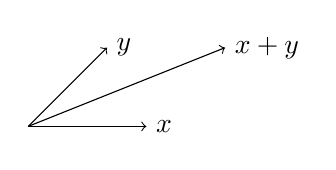
\begin{tikzpicture}
                \draw[->] (0,0) -- (1,1)node[anchor=west]{$y$};
                \draw[->] (0,0) -- (1.5, 0) node[anchor=west]{$x$};
                \draw[->] (0,0) -- (2.5, 1)node[anchor=west]{$x+y$};
            \end{tikzpicture}
            As both sides of the triangle inequality are $\geq0$, square both sides.
            \begin{align}
                |x+y|^2&\stackrel{?}{\leq}(|x|+|y|)^2\\
                \langle x+y, x+y \rangle&\stackrel{?}{\leq}|x|^2+|y|^2+2|x||y|\\
                \langle x,x\rangle + 2\langle x,y\rangle + \langle y,y\rangle &\stackrel{?}{\leq}|x|^2+|y|^2+2|x||y|\\
                |x|^2+|y|^2+2\langle x,y\rangle &\stackrel{?}{\leq}|x|^2+|y|^2+2|x||y|\\
                \langle x,y\rangle &\stackrel{?}{\leq}|x||y|\label{220}
            \end{align}
            \eqref{220} is true by cauchy-schwarz.
            \item The proof is trivial because you can expand the right hand side.
            \\\textbf{Note:} The inner product and the norm are not independent. If you know how to compute one, you can compute the other.
        \end{enumerate}
    \end{proof}
\end{proposition}
\subsection{Distance Functions}
\begin{definition}
    If $x, y\in\R^n$,define the distance between $x\&y$
    \begin{equation}
        d(x,y)=|x-y|
    \end{equation}
\end{definition}
\begin{theorem}
    \begin{enumerate}
        \item $d$ is symmetric: $d(x,y)=d(y,x)$
        \item $d$ is positive definite: $d(x,y)\geq0$ and $d(x,y)=0\iff x=y$
        \item Triangle inequality: $d(x,z)\leq d(x,y)+d(y,z)$
    \end{enumerate}
    The significance of this theorem is that this is all we need to know about distances to comment on continuity.\\
    \textbf{Aside:} Later, this theorem will become a definition for a distance function or a metric.
    \begin{proof}
        \begin{enumerate}
            \item \begin{align}
                d(x,y)=|x-y|=|-(y-x)|=|-1||y-x|=|y-x|=d(y,x)
            \end{align}
            \item \begin{align}
                d(x,y)=0\iff |x-y|=0\iff x-y=0\iff x=y
            \end{align}
            \item \begin{align}
                |x-z|\stackrel{?}{\leq}|x-y|+|y-z|
            \end{align}
            This is true by the previous triangle inequality, $|p|+|q|\geq|p+q|$. Letting $p=x-y,q=y-z\implies p+q=x-z$.
        \end{enumerate}
    \end{proof}

    There are other norms and distance functions that we will rarely use.

    \begin{itemize}
        \item The euclidian norm which we use is $|x|_{L^2}=\sqrt{\sum x_i^2}$.
        \item There is a L1 norm $|x|_{L^1}=\sum|x_i|$.
        \item The L-infinity norm is $|x|_{L^\infty}=\max |x_i|$.
    \end{itemize}
    The distance functions for these norms also satisfys these three properties.
\end{theorem}

\begin{itemize}
    \item There is a bijection between linear maps from $\R^n\to\R^m$ and the set of $m\times n$ matrices with real coefficients. This bijection can be realized by choosing a basis. 
    \item In $\R^n$ or $\R^m$, there is a natural basis (the standard basis) $e_i=\begin{pmatrix}
        0\\
        \vdots\\
        1\\
        \vdots\\
        0
    \end{pmatrix}\leftarrow i-$th position
    \item by $A\in M_{m\times n}\to L_A(x)=Ax$, where $x\in\R^n$.
    \item If T is a linear transformation, $M_T=\begin{pmatrix}\:\\
        Te_1|Te_2|\dots|Te_n\\\:
    \end{pmatrix}$
\end{itemize}
\begin{definition}
    Homomorphism: A map that preserve the structure.
\end{definition}
\begin{theorem}
    \begin{enumerate}
        \setcounter{enumi}{-1}
        \item Bijective
        \begin{align}
            L_{(M_T)}=T, M_{(L_A)}=A
        \end{align}
        \item \begin{itemize}
            \item $A\to L_A$ is linear: $L_{aA+bB}=aL_A+bL_b$
            \item $T\to M_T$ is linear: $M_{aT+bS}=aM_T+bM_S$
        \end{itemize}
        \item Given $T: \R^n\to\R^m, S:\R^m\to\R^p$, and $S\circ T\equiv T//S: \R^n\to\R^p$.\\
        Then, $M_SM_T=M_{S\circ T}$.
    \end{enumerate}
\end{theorem}

End of the review.

\section{Rectangles}
\begin{itemize}
    \item It is common to use intervals in $\R$. In $\R^n$, we use rectangles. 
    \item To specify a rectangle, we must bound the each of the $n$ coordinates.
\end{itemize}
\begin{definition}
    Given $a_i\leq b_i$, where $i=1,\dots, n$,
    \begin{itemize}
        \item The closed rectangle corresponding to $a_i,b_i$ is defined as
        \begin{align}
            R=\prod_{i=1}^n[a_i,b_i]=\{x\in\R^n:\forall i\:\: a_i\leq x_i\leq b_i\}
        \end{align}
        \item The opened rectangle defined by $a_i,b_i$ is defined as 
        \begin{align}
            R=\prod_{i=1}^n(a_i,b_i)=\{x\in\R^n:\forall i\:\: a_i<x_i<b_i\}
        \end{align}
    \end{itemize}
\end{definition}
\begin{itemize}
    \item If $X\&Y$ are sets, we define (from set theory) the cartesian product $X\times Y=\{(x,y): x\in X,y\in Y\}$
    \item Given 3 sets, the cartesian product is strictly speaking not associative as $((x,y),z)\neq(x,(y,z))$. However, for convinence we agree that $((x,y),z)=(x,y,z)=(x,(y,z))$. Thus, the cartesian product is associative.
    \item $\R^n=\R\times\R\times\dots\times\R=\{(x_1,\dots,x_n):x_i\in\R\}$.
\end{itemize}
\begin{definition}
    \begin{itemize}
        \item $A\subset\R^n$ is called an open set if $\forall a\in A\exists$ an open rectangle $R: x\in R\subset A$.
        \item $A\subset\R^n$ is called an open set if $\forall a\in A\exists$ an open ball $B: x\in B\subset A$. An open ball $B=B_r(x_0)=\{y\in\R^n:|x_0-y|<r\}$ Note an open ball can be defined with any norm.
    \end{itemize}
\end{definition}

\begin{theorem}
    Defining ``open'' using rectangles is equivalent to define ``open'' using balls.
    \begin{proof}
        $\implies$ Every open rectangle is open using the ball definition.
        
        $\impliedby$ Every open ball is open using the rectangle definition.
    \end{proof}
\end{theorem}

\begin{definition}
    A set $B$ is ``closed'' if $\R^n \ B=B^C$ is open. 
\end{definition}

\begin{proposition}[\textbf{De-Morgan's Laws}]
   
    If $Y_\alpha$ is any collection of subsets of some universe $U$,
    \begin{align}
        \left(\bigcup Y_\alpha\right)^C&=\bigcap Y_\alpha^C\\
        \left(\bigcap Y_\alpha\right)^C&=\bigcup Y_\alpha^C
    \end{align}
\end{proposition}
\begin{theorem}
    \begin{enumerate}
        \item $\emptyset,\R^n$ are clopen.
        \item Any union of open sets is open. Any intersection of closed sets is closed.
        \item A finite intersection of open sets is open. A finite union of closed sets is closed.
    \end{enumerate}
    \begin{proof}
        \begin{enumerate}
            \item $\R^n$ is open. $x\in\prod(x_i-1,x_i+1)\subset\R^n$. $\implies\emptyset$ is closed. The empty set has no points, thus the condition holds. ``Every horse in an empty set of horses has horns.'' $\implies\R^n$ is closed.
            \item Suppose $\{A_\alpha\}_{\alpha\in I}$, where $I$ is an arbiturary indexing set, is a collection of open sets.
            \begin{equation}
                A=\bigcup_{\alpha\in I}A_{\alpha}=\{x:\exists\alpha\in I\:\:x\in A_\alpha\}
            \end{equation}

            Let $x\in A$, find $\alpha$ such that $s\in A_\alpha$. Find an open rectangle $R$ such that $x\in R\subset A_\alpha\subset A$

            Suppose $\{B_\alpha\}_{\alpha\in I}$ is a collection of closed sets, show $\cap B_\alpha$ is closed.
            $\left(\bigcap B_\alpha\right)^C=\bigcup B_\alpha^C$ is open $\implies\bigcap B_\alpha^C$ is closed.
            \item \begin{lemma}
                The intersection of two open rectangles, if non-empty, is an open rectangle.
            \end{lemma}
            Suppose $A_1$ and $A_2$ are open. Pick $x\in A_1\cap A_2$. By openness of $A_1$, $x\in A_1\implies\exists R_1: x\in\R_1\subset A_1$. Similarly, by openness of $A_2$, $x\in A_2\implies\exists R_2: x\in\R_2\subset A_2$. Then, $x\in R_1\cap R_2\equiv R\subset A_1\cap A_2$.

            Suppose $A_i$, $i=1,\dots,n$ are open.
            \begin{equation}
                \bigcap_{i=1}^n A_i=\left(\bigcap_{i=1}^{n-1}A_i\right)\bigcap A_n
            \end{equation}
            By induction hypothesis, $\left(\bigcap_{i=1}^{n-1}A_i\right)$ is an open set. The intersection of two open sets are open $\implies$ the intersection of $n$ open sets are open.

            Suppose $B_i$, $i=1,\dots,n$ is closed,
            \begin{equation}
                \left(\bigcup_{i=1}^nB_i\right)^C=\bigcup_{i=1}^nB_i^C
            \end{equation}        
        \end{enumerate}
    \end{proof}
\end{theorem}
\begin{definition}
Clopen Sets:
    Suppose $A\subset\R^n$ is clopen $\implies$ $A^C$ is clopen. Suppose neither is empty. 

    Consider the line segment $l_{xy}(t)=ty+(1-t)x$.
    \begin{align}
        l_{xy}(0)&=x\in A\\
        l_{xy}(1)&=y\in A^C\\
        t_0&=\sup_{t\in[0,1]}\{l_{xy}(t)\in A\}\\
        l_{xy}(t_0)&=z
    \end{align}
    if $z\in A$, the rectangele containing $z\cap l_{xy}$ includes $l(t_0+\epsilon)\in A^C$ for some $\epsilon$.

    Similarly if $z\in A^C\implies$ one of $A$ and $A^C$ is not clopen so the other one isn't clopen either. 

    Thus, the only clopen sets is $\emptyset$ and $\R^n$
\end{definition}
\begin{itemize}
    \item Consider the following example,
    \begin{equation}
        \bigcap_{n>0}\left(-\frac{1}{n},1+\frac{1}{n}\right)=[0,1]
    \end{equation}
    This infinite intersection of open sets is not an open set due to the points $0$ and $1$.
\end{itemize}
\begin{definition}
    Given $A\subset\R^n$ and $x\in\R^n$, there is a tricotomy (\textbf{exactly} one of the following is true)
    \begin{enumerate}
        \item $x$ belongs to the \textit{interior} of $A$: $\exists$ open rectangle $R$ such that $x\in R\subset A$.
        \item $x$ belongs to the \textit{exterior} of $A$: $\exists$ open rectangle $R$ such that $x\in R\subset A^C$.
        \item $x$ belongs to the \textit{boundary} or $A$: Every open rectangle $R$ such that $x\in R$ has $R\cap A^C\neq\emptyset$ AND $R\cap A\neq\emptyset$.
    \end{enumerate}
    \begin{itemize}
        \item The closure of $A$ is the complement of the exterior. $\overline{A} = (\mathrm{ext} A)^C$. It will satisfy either condition 1 or 3.
        \item \textbf{Claims: } 
        \begin{enumerate}
            \item $\overline A\ni x$ iff. every open rectangle $R\ni x$ satisfies $R\cap A\neq\emptyset$.
            \item $\mathrm{int} A\cup\mathrm{ext} A\cup \mathrm{Bd} A=\R^n$
            \item $\mathrm{cl} = A\cup\mathrm{Bd} A$
            \item $\mathrm{int} A=A\setminus \mathrm{Bd}A$.
            \item $\mathrm{int} S$ is the largest open set in $S$, $\mathrm{int} S=\bigcup_{U\subset S}U$
            \item $\overline{S}$ is the smallest closed set containing $S$, $\overline{S}=\bigcap_{C\supset S}C$.
        \end{enumerate}
    \end{itemize}
\end{definition}
\begin{example}
    $A=[0,1)\subset \R$
    \begin{itemize}
        \item $\mathrm{int} A=(0,1)$
        \item $\mathrm{ext} A=(-\infty,0)\cup(1,\infty)$
        \item $\mathrm{Bd} A= \{0,1\}$
        \item $\mathrm{cl} A=[0,1]$
    \end{itemize}
\end{example}
\section{Compactness}
\begin{definition}
    An \textbf{open cover} of a set $A$ is a collection $\{U_\alpha\}$ of open sets in $\R^n$ such that 
    \begin{equation}
        \bigcup_{\alpha\in I}U_\alpha\supset A
    \end{equation}

    A \textbf{subcover} of $\{U_\alpha\}_{\alpha\in I}$ is a collection $\{U_\alpha\}_{\alpha\in I'}$ where $I'\subset I$ such that 
    \begin{equation}
        \bigcup_{\alpha\in I'}U_\alpha\supset A
    \end{equation}
\end{definition}
\begin{definition}
    A set $A$ is called \textbf{compact} if \textbf{EVERY} open cover of $A$ has a finite sub-cover.
    \begin{itemize}
        \item Note: Showing one finite open cover with a finite subcover is not sufficient.
    \end{itemize}
    Examples:
    \begin{enumerate}
        \item If $F\subset\R^n$ is finite, then it is compact.
        \item $\R$ is not compact. Take $\R=\bigcup_{n\in\Z}(n-1,n+1)=\bigcup_{n\in\Z}(-n,n)$. These open covers does not have a finite subcover.
    \end{enumerate}
\end{definition}

\subsection{Finding all compact subsets of $\R^n$}
\begin{theorem}[Heine-Borel]
    $[a,b]$ is compact.
    \begin{proof}
        Let $\{U_\alpha\}_{\alpha\in J}$ be an open cover of $[a,b]$. We will first show there's a subcover from a to $g>a$.

        \vspace{10pt}
        Define $G=\{g\in[a,b]: \exists J'\subset J\}$ such that $J'$ is a finite subcover of $[a,g]$.

        \vspace{10pt}
        To show $b\in G$ will prove the theorem. Set $\gamma=\sup G$. For $G$ to have a supremum, it must be bounded ($G\subset[a,b]$) and non-empty ($a\in G$). 

        \vspace{10pt}
        Claim: $\gamma=b$. Suppose $\gamma<b$, as $\gamma\in [a,b]$, $\exists\beta\in J$ such that $\gamma\in U_\beta$.

        \vspace{10pt}
        As $U_\beta$ is open, $\exists (g',g''): \gamma\in(g',g'')\subset[g',g'']\subset U_\beta$.

        \vspace{10pt}
        $[a,g'']=[a,g']\cup[g',g'']$.

        As $g'<\gamma$, $[0,g']$ has a finite subcover. $[g',g'']$ is covered by a single set $U_\beta$. Thus, $g''\in G$ and this is a contradiction as $g''>\gamma$.


        Next, we show $b=\gamma\in G$. 

        If $b$ is covered by $\{U_\alpha\}_{\alpha\in J}$, hence some interval $(b^-,b^+)$ is covered by one set $U_\alpha$. As $\sup G=b>b^-, \exists g'\in G: b^-<g'<b$.
        \begin{equation}
            [a,b]=[a,g']\cup[b^-,b]
        \end{equation}
    \end{proof}
\end{theorem}
\begin{theorem}[]
    If $A\subset\R^n$ is compact and $b\subset\R^m$ is compact. Then, $A\times B\subset\R^{n+m}$ is compact.
    \begin{proof}
        Suppose $U=\{U_{\alpha}\}$ is an open cover of $A\times B$.

        \vspace{10pt}
        WLOG, each $U_\alpha$ is itself an open rectangle.
        \vspace{10pt}
                
        \begin{lemma}
            For every $x\in A$, we can find an open set $N_x\ni x: N_x\times B$ can be covered with finitely many of the $U_\alpha$s.
            \vspace{10pt}
            
            \begin{proof}
                Write $U_\alpha=V_\alpha\times W_\alpha$, where $V_\alpha,W_\alpha$ are open rectangles in $\R^n,\R^m$ respectively.
                
                Consider that $\{W_\alpha:x\in V_\alpha\}$ covers $B$ which is compact. So find $\alpha_1,\dots,\alpha_p: \{W_{\alpha_1},\dots,W_{\alpha_p}\}$ cover $B$. So, $\{U_{\alpha_1},\dots,U_{\alpha_p}\}$ cover $\{x\}\times B$.
                \vspace{10pt}
                
                Let $N_x=\bigcap_{i=1}^pV_{\alpha_i}\subset V_{\alpha_i}\subset V_{\alpha_i}\forall i$.
                \vspace{10pt}

                Now, $N_x\times B\subset\bigcup_{i=1}^pN_x\times W_{\alpha_i}\subset\bigcup_{i=1}^pV_{\alpha_i}\times W_{\alpha_i}=\bigcup_{i=1}^pU_{\alpha_i}$.
            \end{proof} 

        \end{lemma}
    \end{proof}
    Now, $\{N_x\}_{x\in A}$ is an open cover of $A$. By compactness of $A$, find $x_1,\dots,x_q:\bigcup_{j=1}^qN_{x_j}\supset A$. i.e. $\bigcup_{j=1}^qN_{x_j}\times B\supset A\times B$.

    For each $j=1,\dots,q$ find $U_{ji}$ which are rectangles in $U$, $i=1,\dots,p_j:\bigcup_{i=1}^{p_j}U_{ji}\supset N_{x_j}\times B$. 
    
    Now, $\bigcup_{j=1}^p\bigcup_{i=1}^{p_j}U_{ji}\supset A\times B$.
\end{theorem}
\begin{corollary}
    Closed rectangles $R=\prod_{i=1}^n[a_i,b_i]$ are compact.
\end{corollary}
\begin{proposition}
    A closed subset of a compact set is compact. 
\end{proposition}
\begin{corollary}
    Every closed and bounded subset of $\R^n$ is compact.
\end{corollary}

\begin{theorem}
    Every compact set in $\R^n$ is closed and bounded.
    \begin{proof}
        Construct a cover for $S$ with open balls of radius $R$. Given $S$ is compact, it is covered by finitely many elements. Thus, $S$ is bounded.
        
        Let $x\in S^C, y\in S$, Let $B_y=B(y,\frac{1}{3}|x-y|),C_y=B(x,\frac{1}{3}|x-y|)$
    \end{proof}
\end{theorem}

If $X\subset\R^n$ is compact, 
\begin{itemize}
    \item Every open cover has a finite subcover
    \item Closed and bounded
    \item Every sequence $(x_n)_n\in X$ has a converging subsequences that converge in $X$.
\end{itemize}

Continuity:
\begin{itemize}
    \item $\epsilon-\delta$
    \item $f^{-1}(\text{open})$ is open
    \item If $x_n$ converges to x, then $f(x_n)$ converges to $f(x)$.
\end{itemize}

\section{Continuity}

\begin{definition}[Image and Preimage]
    Given $F:\R^n\to\R^m$,
    \begin{itemize}
        \item $C\subset\R^n$, the image of $C$ is $F(C):=\{F(\gamma):\gamma\in C\}$
        \item $D\subset\R^m$, the preimage of $D$ is $F^{-1}(D):=\{\gamma\in\R^n:F(\gamma)\in D\}$
    \end{itemize}
    Note the image behaves better on points, but preimage behaves better on sets, as,
    \begin{align}
        F^{-1}(D_1\cup D_2)&=F^{-1}(D_1)\cup F^{-1}(D_2)\\
        F^{-1}(D_1\cap D_2)&=F^{-1}(D_1)\cap F^{-1}(D_2)\\
        F^{-1}(D^C)&=F^{-1}(D)^C
    \end{align}

    \begin{align}
        F(C_1\cup C_2)&=F(C_1)\cup F(C_2)\\
        F(C_1\cap C_2)&\subset F(C_1)\cap F(C_2)\\
        F(C^C)&\neq F(C)^C
    \end{align}
\end{definition}
\begin{definition}[Projection]
    $\pi_i:\R^n\to\R$
    \begin{equation}
        \pi_i\begin{pmatrix}
            x_1\\\vdots\\x_n
        \end{pmatrix}=x_i
    \end{equation}
\end{definition}
\begin{definition}[Coordinate Functions]
    For $F:\R^n\to\R^m$, or 
    \begin{align}
        \begin{pmatrix}
            x_1\\\vdots\\x_n
        \end{pmatrix}\to\begin{pmatrix}
            y_1\\\vdots\\y_m
        \end{pmatrix}=\begin{pmatrix}
            f_1(x_1,\dots,x_n)\\\vdots\\f_m(x_1,\dots,x_n)
        \end{pmatrix}
    \end{align}

    Where $f_i:\R^n\to\R$ for $i=1,\dots,m$ are the coordinate functions of $f$. $f_i=\pi_i\circ F$ 
\end{definition}
\begin{definition}[Composition]
    Given $f:\R^n\to\R^m$, $g:\R^m\to\R^p$, and $h=g\circ f:\R^n\to\R^p$
    \begin{equation}
        h(x)=g(f(x))=(g\circ f)(x)
    \end{equation}
\end{definition}
\begin{definition}[Graph]
    A function $f:\R\to\R$, the graph of $f$ is 
    \begin{equation}
        \Gamma_f=\{(x,f(x)):x\in\R\}\subset\R\times\R=\R^2
    \end{equation}

    A function $f:\R^n\to\R^m$, the graph of $f$ is 
    \begin{equation}
        \Gamma_f=\{x,f(x):x\in\R^n\}\subset\R^n\times\R^m=\R^{n+m}
    \end{equation}
\end{definition}
\begin{definition}[Limit]
    Suppose $f:A\subset\R^n\to\R^m;a\in\overline A$
    \begin{equation}
        \lim_{x\to a}f(x)=b \text{ means } \forall\varepsilon>0\exists\delta>0:x\in (B_\delta(a)\setminus\{x\})\cap A\implies f(x)\in B_\epsilon(b)
    \end{equation}

    \begin{itemize}
        \item If the limit exists, it is unique.
    \end{itemize}
\end{definition}
\begin{definition}[Continuity]
    $f:A\subset\R^n\to\R^m$ is continuous at $a\in A$ if $\lim_{x\to a}f(x)=f(a)$.

    $f$ is continuous on $A\iff f$ is cont. at every $a\in A$.
    \begin{equation}
        \iff\forall a\,\forall\epsilon>0\,\exists\delta>0\,\forall x\in A:|x-a|<\delta\implies|f(x)-f(a)|<\epsilon
    \end{equation}
\end{definition}
\begin{definition}
    $B\subset A$ is \textit{open in }$A$ if $\exists U$ open in $\R^n$ such that $B=U\cap A$.
\end{definition}
\begin{theorem}
    \begin{enumerate}
        \item $f:\R^n\to\R^m$ is cont. iff for every open set $V\subset\R^m, f^{-1}(V)$ is also open.
        \item $f:A\subset\R^n\to\R^m$ is cont. iff for every open set $V\subset\R^m, f^{-1}(V)$ is open in $A$.
    \end{enumerate}
\end{theorem}


\end{document}
